\documentclass[10pt]{article}

\usepackage[margin=0.82in]{geometry}
\usepackage{amsmath}
\usepackage{booktabs}
\usepackage{float}
\usepackage{graphicx}
\usepackage{microtype}
\usepackage[numbers,sort&compress]{natbib}
\usepackage{needspace}
\usepackage{placeins}
\usepackage[hidelinks]{hyperref}
\usepackage{xcolor}

\hypersetup{
  pdftitle={Selective Authorization of Automated Performance Patches: Rule Audit and Case Study of a Frozen Promotion Gate},
  pdfauthor={Junming Liang},
  pdfsubject={Technical Report v0.1, September 2026}
}

\newcommand{\NullCount}{30}
\newcommand{\NullPromotions}{0}
\newcommand{\NullUpperBound}{9.503\%}
\newcommand{\NaiveNull}{16/30}
\newcommand{\BootstrapNull}{2/30}
\newcommand{\TotalPairs}{252}
\newcommand{\NullPairs}{244}
\newcommand{\RealPairs}{8}
\newcommand{\RealGainMs}{35.861}
\newcommand{\RealControlMs}{550.473}
\newcommand{\RealGainPct}{6.515\%}
\newcommand{\RealCiLow}{6.368}
\newcommand{\RealCiHigh}{58.506}
\newcommand{\RealPValue}{0.030985}
\newcommand{\RealSign}{0.875}
\newcommand{\QMinimumN}{29}
\newcommand{\DirectCiRatio}{9}

\title{Selective Authorization of Automated Performance Patches:\\
Rule Audit and Case Study of a Frozen Promotion Gate}
\author{Junming Liang\\Anhui Normal University}
\date{Technical Report v0.1 -- September 2026}

\begin{document}
\maketitle

\begin{abstract}
Coding agents can propose performance patches faster than noisy hardware can
validate them.  This creates an authorization problem distinct from patch
generation: when is the evidence strong enough to permit automatic promotion?
We audit a frozen promotion gate rather than proposing a post-hoc replacement.
Its direct path combines a practical-effect estimand with an uncalibrated
directional-consistency threshold.  Under an IID Bernoulli-sign interpretation,
certifying $q>0.9$ with a one-sided 95\% lower bound requires at least
$n=\QMinimumN$ observations and, at that minimum, every paired difference must
be positive; the frozen ladder stops at 4/8/12.  Arm order is also perfectly
confounded with pair-index parity, so an order effect is not identifiable.

The accompanying preregistered public case study evaluates the gate on fmt
12.1.0 using 30 strict A/A null candidates and one real buffer-reuse candidate.
The gate promoted \NullPromotions{} of \NullCount{} nulls; under an independent,
common-probability Bernoulli model, the corresponding one-sided 95\% upper bound
is \NullUpperBound{}.  All null candidate and control binaries were
byte-identical and shared one hash, so this result calibrates the complete
pipeline on strict A/A inputs rather than on semantically equivalent but
binary-distinct patches.  A deliberately weak first-pair counterfactual would
have accepted \NaiveNull{} nulls.  The real candidate showed a median paired
gain of \RealGainMs{} ms (\RealGainPct{}) but ended as
\texttt{accepted\_noisy\_single}, an evidence-only verdict requiring
independent replication.  The report contributes a claim-bounded rule audit,
a reproducible case study, and a preregistered design for a later
authorization-frontier study; it does not claim a universal false-promotion
rate, a superior gate, or cross-system generality.
\end{abstract}

\noindent\textbf{Scope.} The next-stage simulation contract is unexecuted; all
related policy comparisons are prospective.

\section{Introduction}

Performance optimization is increasingly treated as a long-horizon coding
agent task.  Recent systems learn or generate performance-improving edits
across programs and repositories~\citep{shypula2024}.  Generation, however,
does not settle whether a proposed patch should be merged.  Runtime evidence
on shared hardware is affected by process noise, host state, and multilevel
variation; rigorous benchmarking therefore requires explicit experimental
units, repetition, and uncertainty rather than one favorable timing
observation~\citep{georges2007,kalibera2013}.  Automated tuning under unstable
measurements faces the same problem~\citep{tuna2025}.

We study a narrower decision: \emph{when should an automated system receive
authority to promote a performance patch?}  Candidate generation and promotion
are different roles.  A search procedure may produce many speculative edits,
while a promotion authority must fail closed when correctness, practical
effect, or measurement quality is unresolved.  This distinction is especially
important when a statistically interesting result remains too noisy for an
unattended merge.

The case study freezes one promotion procedure before timing and evaluates it
on one public C++ target.  Thirty strict null candidates provide an empirical
calibration of end-to-end false promotion behavior.  One real buffer-reuse
candidate checks that the procedure is not evaluated only on nulls.  The
design uses paired candidate/control observations, a bootstrap interval, a
paired permutation statistic, a minimum practical effect, a directional
consistency filter, host-weather gating, and bounded escalation.  These are
established statistical and measurement components, not individually claimed
as methodological inventions~\citep{efron1993,good2005}.

This report makes four claim-bounded contributions:
\begin{enumerate}
  \item It audits the frozen authorization semantics.  The direct path conjoins
  an effect threshold with directional consistency without a stated joint
  operating-characteristic calibration, and a $q>0.9$ confidence
  interpretation is infeasible within the frozen 4/8/12 ladder under the IID
  binomial model.
  \item It reports a fully replayable public case study: \NullPromotions{} of
  \NullCount{} strict A/A nulls were promoted, while a real candidate was
  retained as evidence but not automatically promoted.  All null candidate
  and control binaries were byte-identical, so the null result calibrates this
  end-to-end A/A pipeline rather than behavior on binary-distinct semantic
  nulls.
  \item It shows why binary identity is part of the result rather than an
  implementation detail.  A strict A/A calibration with identical binaries
  cannot measure sensitivity to layout or alignment changes in semantically
  equivalent, binary-distinct patches; such studies should report whether the
  timed artifacts actually differ.
  \item It identifies a design limitation: deterministic alternation makes arm
  order a function of pair-index parity, preventing identification of an arm
  order effect.  Sequence diagnostics are reported only as post-hoc
  exploratory evidence.
\end{enumerate}

The contribution is consequently not ``a new bootstrap gate.''  It is an
empirical and analytical audit of how a concrete automated promotion policy
allocates authority, abstention, and replication.  A later, separately frozen
study will compare alternative policies across risk, power, abstention, and
cost; no such frontier is claimed here.

\section{Related Work}

Prior work shows that performance evidence can be distorted before any
decision rule is applied.  Mytkowicz et al.~\citep{mytkowicz2009} document how
seemingly innocuous experimental choices can produce wrong performance data.
STABILIZER~\citep{curtsinger2013} addresses this class of problem with
randomization and a statistically grounded measurement methodology.  Duet
Benchmarking~\citep{bulej2020duet} studies interference-aware measurement in
the cloud, where co-running activity can obscure the effect of the program
under test.  These works motivate the present emphasis on paired observations,
host weather, and explicit uncertainty, but they do not specify when a system
should be granted authority to promote a code edit.

At a larger operational scale, FBDetect~\citep{yoon2024fbdetect} targets tiny
performance regressions through in-production monitoring at Meta.  Its unit of
concern is regression detection across a production fleet; the unit here is a
candidate patch entering an automated promotion pipeline under a bounded
measurement budget.  The distinction is consequential: a detector may identify
a likely regression without defining a policy for abstention, independent
replication, or automatic authorization.  This report therefore treats the
preceding systems as measurement and detection neighbors, not as competing
promotion gates.  Its contribution is to make the authorization semantics of a
concrete frozen gate explicit and auditable, while leaving any replacement
policy to a separately frozen study.

\paragraph{Relationship to a companion manuscript.}
The gate audited here is the same frozen \path{paired_bootstrap_permutation_v1}
judge that an earlier manuscript by the same author, unpublished at the time of
writing, evaluates on a different subject.  That manuscript asks whether such a
gate can hold a low promotion rate under noise, and its principal arm uses a
constructed candidate set whose candidate-level rows are withheld.  This report
asks a different question -- what the decision rule can and cannot certify --
on a separately preregistered study whose subject is fmt 12.1.0 and whose
complete candidate-level evidence is released.  The two share a measurement
methodology and an author; they do not share a subject program, a measurement
run, or any candidate-level evidence.

\section{Audited Promotion Procedure}

\subsection{Authority and outcomes}

The procedure separates search from promotion.  A candidate first has to pass
the frozen semantic correctness contract.  It is then timed against a control
inside the same locked host window.  A positive paired difference
$d_i=t_{i,\mathrm{control}}-t_{i,\mathrm{candidate}}$ indicates that the
candidate was faster.

The frozen public judge can emit three operational classes relevant here:
\begin{itemize}
  \item \texttt{accepted}: direct automatic promotion;
  \item \texttt{accepted\_noisy\_single}: statistically positive but noisy
  evidence, retained for an independent replication and not promoted;
  \item \texttt{NOISY\_PENDING} or \texttt{rejected}: no promotion authority
  from the current run.
\end{itemize}
An independently replicated noisy signal may later become
\texttt{accepted\_noisy\_replicated}, which is a promotion verdict.  This study
did not authorize or execute that replication.

\subsection{Frozen statistics and ladder}

At a decision depth, the judge computes the median paired improvement
$\widehat\theta$, a two-sided 95\% bootstrap interval $[L,U]$, a paired
permutation $p$-value, and the fraction of pair signs agreeing with the sample
median.  The minimum practical effect is
\begin{equation}
  \delta_{\min}=0.005\,\widetilde t_{\mathrm{control}}.
\end{equation}
The interval margin, width, and decisiveness are
\begin{equation}
  M=L-\delta_{\min},\qquad W=U-L,\qquad K=M/W.
\end{equation}
The direct, \emph{decisive} confidence tier requires
\begin{equation}
  M>0,\qquad K\ge 1.0,\qquad
  \widehat q_{\mathrm{match}}\ge 0.9.
  \label{eq:decisive}
\end{equation}
A \emph{marginal} tier requires $M>0$ and permutation $p\le0.05$.
Marginal evidence on a noisy host can become
\texttt{accepted\_noisy\_single}; it is not direct promotion.

The sample ladder is m4, m8, and m12.  m4 is screening-only and has no terminal
promotion authority.  m8 is the first formal decision, while m12 is reached
only through the frozen escalation rule.  Bootstrap and permutation procedures
use 2,000 resamples each.  Although the interval and permutation components
have nominal settings, the conjunction in Equation~\ref{eq:decisive}, the
data-dependent ladder, and the replication route were not jointly calibrated
to a stated false-authorization probability.

\subsection{Counterfactuals}

The preregistered \emph{naive-k1} counterfactual accepts whenever the first
paired difference is positive.  It is intentionally weak and is not presented
as a competitive statistical baseline.  A separate bootstrap-only sensitivity
accepts when the final 95\% bootstrap interval has $L>0$.  The latter analysis
was defined after the experiment and is therefore labeled post-hoc
exploratory.  It omits the practical-effect margin, permutation evidence,
directional consistency, and decisiveness requirements.

\section{Study Design}

\subsection{Subject and workload}

The public subject is fmt 12.1.0 at source commit
\texttt{407c905e45ad75fc29bf0f9bb7c5c2fd3475976f}.  The frozen wrapper performs
1,024,000 formatting operations per process.  Each observation launches a
fresh process of a previously compiled binary.  Candidate and control are
measured as an ordered pair under one validation lock, and candidates execute
sequentially.

The host-weather gate uses five control measurements before candidate timing.
The first attempt was classified \texttt{NOISY} and produced no candidate
observations.  A second attempt was classified \texttt{QUIET} and supplied the
only formal candidate window.  This preserves the failed preflight without
mixing it into the candidate denominator.

\subsection{Strict nulls and real candidate}

The frozen denominator contains \NullCount{} strict null candidates and one
real candidate, \texttt{fmt\_buffer\_reuse}.  The null transformations passed a
pre-timing executable-token equivalence check and, in the compiled formal
artifacts, every null candidate binary was byte-identical to its control.  All
30 nulls also shared the same SHA-256 value beginning
\texttt{6e50bccc4189c8aa}.  The real candidate binary, beginning
\texttt{52d798dec09f688f}, differed from control.

This distinction defines the null estimand.  The null experiment evaluates the
complete measurement and decision pipeline under A/A binary identity.  It does
not estimate false promotion for source changes that preserve semantics while
altering code layout, alignment, or generated machine code.

The real candidate reuses an output buffer to reduce repeated work.  It is a
single functional control, not a power sample or a representative population
of agent-generated patches.  All 31 candidates passed correctness, so this
study confirms execution of the correctness gate but does not estimate its
ability to reject deliberately incorrect candidates.

\subsection{Preregistration, custody, and replay}

The target, source, workload, candidate set, ladder, judge, and denominator
were frozen before formal timing.  The final execution manifest, authorization,
and append-only ledger are bound by SHA-256.  Registration is self-custodied
and hash-bound; it was not deposited with an external registry.  The authorized
run completed all
31 terminal candidate rows.  A later command-line post-processing failure
occurred after measurement completion; recovery regenerated only derived
summary files and recorded that no measurement row changed.

The public v2 package is a typed, derived representation of the frozen custody.
Its self-contained standard-library recomputer reconstructs all 31 terminal
judgments and 63 cumulative stage judgments, verifies pair semantics and
bindings, and fails closed under pair tampering.  It does not import the formal
runner.  The public judge extraction also matches the original judge on 64
fixed-seed differential cases.  This is observed-input and test-matrix
equivalence, not proof of full input-domain program equivalence.

\subsection{Endpoints and uncertainty}

The primary descriptive endpoint is the count of automatic promotions among
the \NullCount{} strict nulls.  For comparison with the frozen report, we also
show a one-sided 95\% Clopper--Pearson upper bound~\citep{clopper1934}.  Its
coverage interpretation requires candidate-level outcomes to behave as
independent Bernoulli draws with a common promotion probability.  Without that
model, the unconditional observation is only the numerator and denominator.

Secondary endpoints are the naive-k1 result, the post-hoc bootstrap-only
sensitivity, the real-candidate outcome, and total paired measurement count.
No fixed-depth cost comparator was preregistered, so pair-count comparisons to
always-m8 or always-m12 are descriptive rather than efficiency estimates.

\section{Frozen Results}

\subsection{Strict-null outcome and its scope}

The frozen gate automatically promoted \NullPromotions{} of \NullCount{} strict
nulls.  Eighteen ended as \texttt{NOISY\_PENDING} and 12 as
\texttt{rejected}; no candidate was removed from the denominator.  Under the
candidate-level independent common-probability Bernoulli model, zero events in
30 trials give the one-sided 95\% upper bound
\begin{equation}
  1-0.05^{1/30}=0.09503,
\end{equation}
or \NullUpperBound{}.  This is not evidence that the population false-promotion
probability is zero.

The binary result must be read beside that numerator: all \NullCount{} null
candidate/control pairs were byte-identical, and all shared one binary hash.
Accordingly, 0/30 is an end-to-end A/A calibration of this implementation.  It
does not establish the gate's behavior on binary-distinct semantic nulls.

\begin{figure}[H]
  \centering
  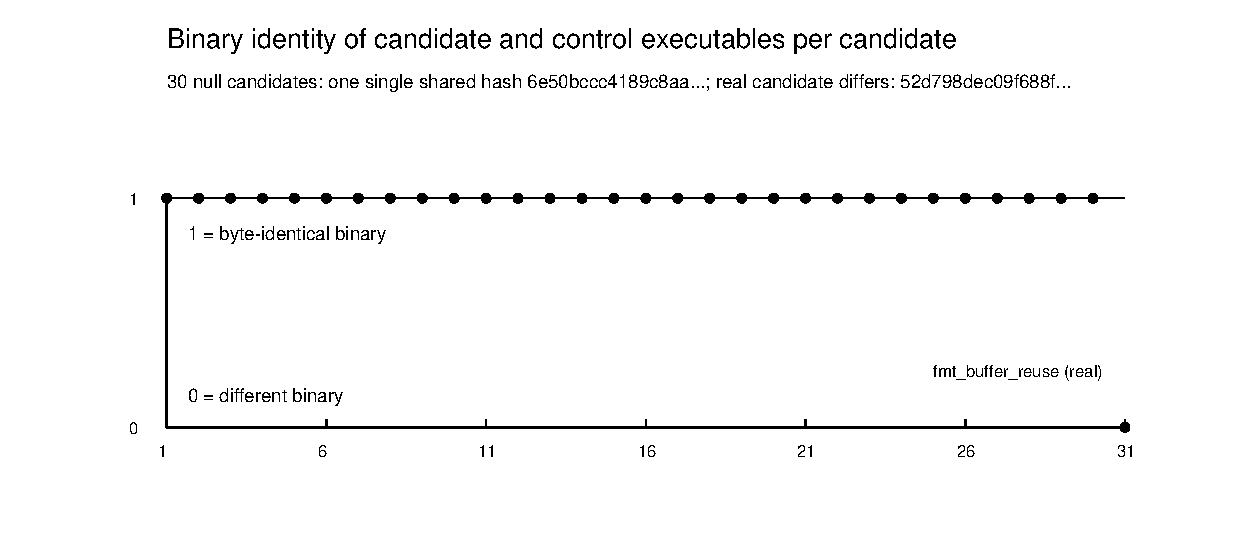
\includegraphics[width=0.88\linewidth]{../../paper_numbers/fig3_binary_hash_contrast.pdf}
  \caption{Binary identity in the frozen denominator.  All 30 strict null
  candidate binaries equal control and share one hash; the real candidate is
  binary-distinct.  The figure describes the tested null class rather than a
  broader semantic-equivalence population.}
  \label{fig:binary}
\end{figure}

\subsection{Counterfactual decisions}

Table~\ref{tab:decisions} compares the frozen result with two explicitly
bounded counterfactuals.  Naive-k1 would have accepted \NaiveNull{} nulls.  It
also missed the real candidate because that candidate's first paired
difference was $-9.387$ ms.  Bootstrap-only accepted \BootstrapNull{} nulls,
\texttt{fmt-011} and \texttt{fmt-016}, and accepted the real candidate.  The
two nulls had interval lower bounds of 2.818 ms and 2.573 ms, but permutation
$p$-values of 0.096952 and 0.112944.  These same-data results illustrate
different filtering behavior; they are not independent estimates of
population error or power.

\begin{table}[H]
  \centering
  \caption{Frozen and counterfactual outcomes.  Bootstrap-only is post-hoc
  exploratory; naive-k1 is a preregistered deliberately weak counterfactual.}
  \label{tab:decisions}
  \begin{tabular}{@{}lcc@{}}
    \toprule
    Rule & Strict-null accepts & Real-candidate result \\
    \midrule
    Frozen promotion gate & 0/30 & signal only; no promotion \\
    Naive-k1 & 16/30 & missed \\
    Bootstrap-only & 2/30 & accepted \\
    \bottomrule
  \end{tabular}
\end{table}

\subsection{Real-candidate evidence}

The real candidate reached m8 with a median paired gain of \RealGainMs{} ms.
Relative to its run-internal control median of \RealControlMs{} ms, this is
\RealGainPct{}.  Its 95\% bootstrap interval was
$[\RealCiLow{},\RealCiHigh{}]$ ms, paired permutation
$p=\RealPValue{}$, and sign consistency \RealSign{}.  The confidence tier was
\texttt{marginal}; the final verdict was
\texttt{accepted\_noisy\_single}.  Thus the procedure retained a positive
signal but did not grant automatic promotion.  No independent replication was
authorized or run.

This single candidate demonstrates that the gate is not evaluated only by
whether it rejects nulls.  It does not estimate recall, establish production
readiness, or show that \RealGainPct{} generalizes across machines and
workloads.

\subsection{Sampling and environment}

The study used \NullPairs{} null pairs and \RealPairs{} real-candidate pairs,
for \TotalPairs{} total.  Thirty candidates terminated at m8; only
\texttt{fmt-011} escalated to m12.  This was four pairs more than always-m8 and
120 fewer than always-m12, but neither fixed-depth policy was a preregistered
comparator, so these differences are not claimed as cost savings.

The rejected preflight had a control CV of 0.1399 and relative range 0.3303;
the accepted quiet preflight had CV 0.0116 and relative range 0.0282.  The
control-only calibration median was 532.686 ms, whereas the real candidate's
run-internal control median was \RealControlMs{} ms, a descriptive 3.339\%
cross-session shift.  All reported gain percentages use the run-internal
paired control, not the earlier calibration value.

\section{Rule Audit}

\subsection{Two quantities in one direct decision}

The interval margin addresses an effect-size quantity: whether the median
paired gain exceeds $\delta_{\min}$.  The sign filter estimates a different
quantity, $q_{\mathrm{match}}$, the probability that a pair has the same sign
as the population median.  A distribution can have median gain above the
practical threshold while fewer than 90\% of individual pair differences are
positive.  Equation~\ref{eq:decisive} therefore embeds a directional-reliability
requirement in the direct authorization path.

That requirement may be a legitimate policy estimand, but the frozen rule
compares only the point estimate $\widehat q_{\mathrm{match}}$ with 0.9.  It
does not use a lower confidence bound for $q_{\mathrm{match}}$, and the public
protocol does not state a separate acceptable error probability for certifying
that quantity.  Conversely, if directional reliability is only diagnostic,
it should not be interpreted as evidence about the median-effect estimand.

\subsection{What the frozen sample budget can certify}

Under IID Bernoulli signs, even an all-positive sequence of length $n$ has the
one-sided 95\% Clopper--Pearson lower bound $0.05^{1/n}$.  Certifying
$q>0.9$ therefore requires
\begin{equation}
  0.9^n\le0.05,
\end{equation}
whose smallest integer solution is $n=\QMinimumN$.  The lower bound is 0.688
at $n=8$, 0.779 at $n=12$, and 0.902 at $n=29$.  Thus, if 0.9 is interpreted as
a confidence-backed directional-reliability requirement, the frozen m4/m8/m12
budget cannot certify it even when every observed sign agrees.  This is a
conditional feasibility statement, not an assertion that the existing point
filter is itself a 5\% test.

\begin{figure}[t]
  \centering
  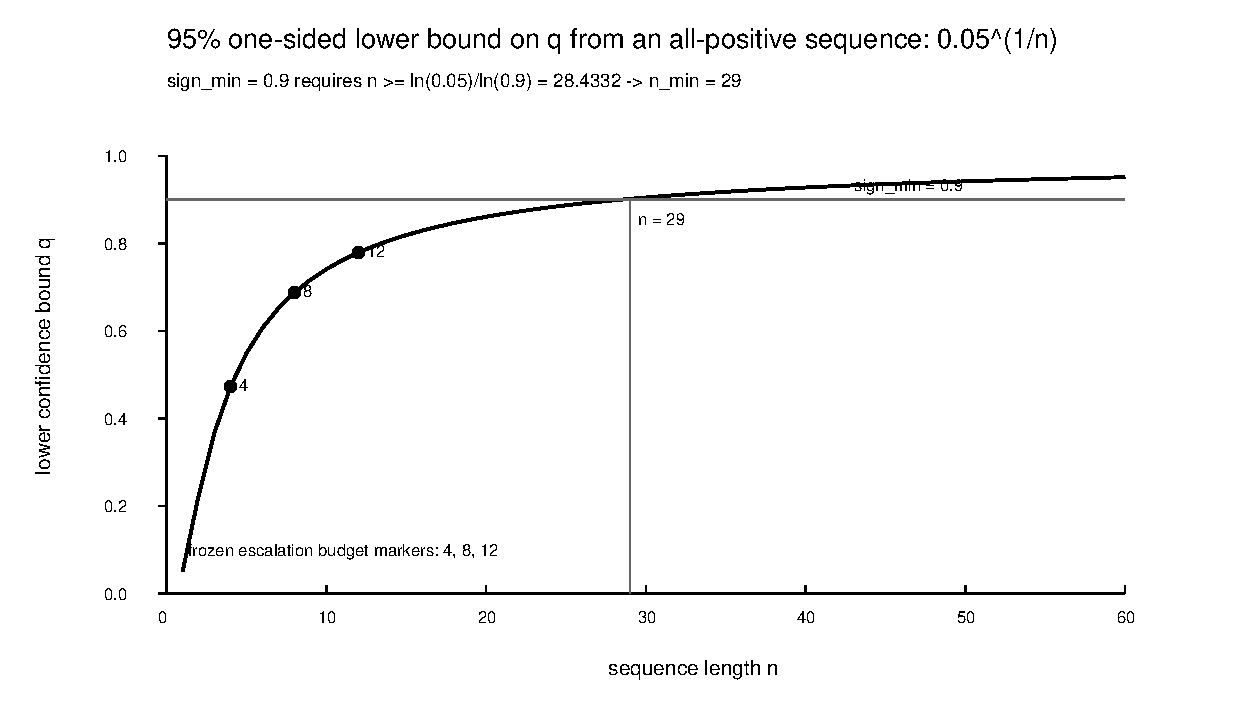
\includegraphics[width=0.88\linewidth]{../../paper_numbers/fig1_signing_lower_bound.pdf}
  \caption{One-sided 95\% lower bound after an all-positive IID Bernoulli
  sequence.  The frozen 4/8/12 budget lies below the first sample size that can
  certify $q>0.9$.}
  \label{fig:qbound}
\end{figure}

\subsection{Implicit evidence premium in the decisive tier}

For a symmetric interval $[\widehat\theta-h,\widehat\theta+h]$, the decisive
condition $M/W\ge1$ implies
\begin{equation}
  \widehat\theta-\delta_{\min}\ge3h.
\end{equation}
Using $h\approx1.96\,\mathrm{SE}$ gives an approximate decisive crossing at
5.88 standard errors, compared with 1.96 standard errors for the interval
margin $L>\delta_{\min}$.  Under a common $1/\sqrt n$ scaling, the corresponding
single-stage sample-count ratio is approximately
$({5.88}/{1.96})^2=\DirectCiRatio{}$.

This calculation is interval geometry, not a complete path-cost comparison.
It excludes the permutation condition, sign consistency, discrete ladder,
bootstrap-median behavior, and the cost and joint success probability of an
independent replication.

\begin{figure}[H]
  \centering
  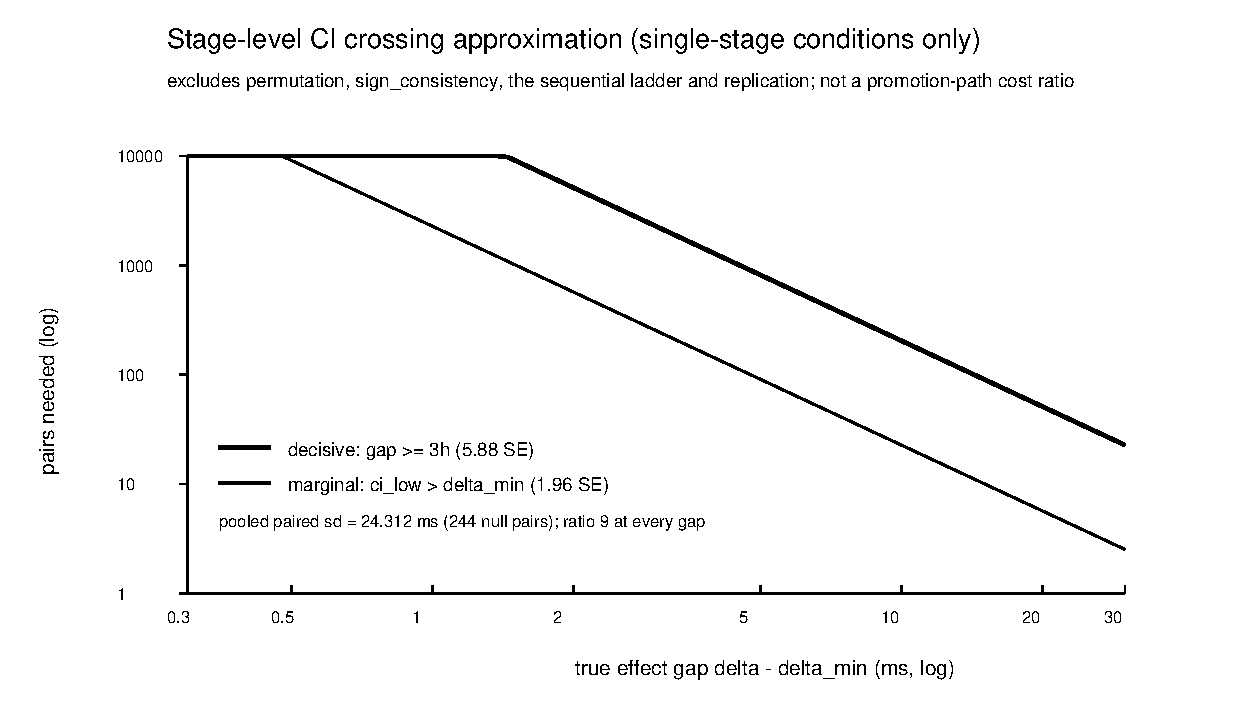
\includegraphics[width=0.88\linewidth]{../../paper_numbers/fig2_stage_level_ci_crossing.pdf}
  \caption{Analytical single-stage CI-crossing approximation using the null-pair
  scale reported by the deterministic figure generator.  The curves are not
  empirical power and do not represent total direct-versus-replication cost.}
  \label{fig:crossing}
\end{figure}

\Needspace{9\baselineskip}
\subsection{Discrete exact-test reference}

As a reference rather than a proposed replacement, an exact one-sided binomial
test of $P(d>\delta_{\min})>0.5$ has actual size below its nominal 0.05 level
because of discreteness.  Across every integer $n$ from 8 through 60, the
actual IID size ranges from 0.0107 to 0.0494, with mean 0.0347.  Reporting power
without these changing realized sizes would confound conservatism with policy
quality.  This reference also answers a different question from the frozen
$\widehat q_{\mathrm{match}}\ge0.9$ filter.

\FloatBarrier
\section{Threats to Validity}

\paragraph{Null class and subject scope.}
The 30 nulls are strict A/A binaries, not binary-distinct semantic nulls.  The
study has one library, workload, machine, quiet window, and real candidate.
Neither the numerator nor the real-candidate result supports cross-project or
cross-machine generalization.

\paragraph{Candidate-level probability model.}
The \NullUpperBound{} upper bound assumes independent candidate-level Bernoulli
outcomes with a common probability.  Candidates were executed sequentially on
one host, so 0/30 is the primary unconditional fact.  The interval is a
model-based summary, not a universal guarantee.

\paragraph{Order and dependence.}
Odd pair indices always ran candidate first and even indices always ran control
first: 0 of \NullPairs{} null pairs violated this mapping.  Arm order is thus
perfectly confounded with parity, and an arm-order effect is not identifiable.
Future paired studies should randomize or counterbalance arm order independently
of pair-index parity and record the realized order.
Post-hoc sequence diagnostics find more sign alternation than a
within-candidate permutation reference, but lag one was selected after the
order structure was observed and multiplicity was not controlled.  These
diagnostics provide exploratory evidence against a naive exchangeability
interpretation; they neither identify a mechanism nor prove IID failure.

\paragraph{Rule audit.}
The $n=29$ result is exact only under IID Bernoulli signs.  The 9-fold result is
a symmetric-normal CI-crossing approximation.  Neither is a measured
risk--power--cost frontier.  No alternative rule has been shown superior.

\paragraph{Selection and replication.}
The real candidate is one selected functional control.  Its observed gain is
not an unbiased estimate of performance across candidate-generating systems.
The required independent replication was not run, so the study cannot report
confirmation probability or post-selection shrinkage.

\section{Next-Stage Design}

A committed draft simulation contract specifies a later comparison of seven
policy families across effect, directional reliability, distribution shape,
dependence, and budget.  It separates the median-effect estimand from
directional consistency, includes IID, block-dependent, and period-2 data
generating processes, and requires replay, analytical, and differential
self-checks.  The dependence parameters remain intentionally unfrozen pending
the exploratory audit.

The contract is a design artifact, not a result.  No Monte Carlo grid has been
run, no policy has qualified, and this report makes no recommendation to change
the frozen gate.  A later version may report a selective-authorization frontier
only after the contract is independently reviewed and frozen.

\section{Artifact Availability}

The public artifact contains typed pair-level evidence, the extracted frozen
judge, fixed differential cases, custody and inventory hashes, a self-contained
recomputer, and an external-consumer acceptance record.  The v0.1 number
reproducer independently emits every value used in this report and states the
criterion and assumptions for each claim.  The pair-dependence audit and all
three figures are deterministic under their recorded inputs and seeds.

\paragraph{AI-assisted research provenance.}
AI coding assistants supported repository implementation, evidence checking,
and manuscript drafting.  The public package does not retain
candidate-by-candidate model attribution or raw agent logs, so this report
does not claim
that every fmt candidate was agent-generated.  Interface model labels, where
reported outside the publication package, are dated, author-reported provenance
rather than machine-bound experimental factors.  The author retained authority
over protocol definition and freeze, execution authorization, interpretation,
and every claim.  Numerical values were accepted only when reproduced by the
deterministic public recomputer and the v0.1 number-reproduction script; no
model-generated number is treated as evidence.

Private host paths, raw agent logs, lock commands, and untracked evidence are
excluded from the publication trees.  A recursive scanner verifies the public
v1 and v2 packages and reports only redacted finding categories for the private
evidence tree.

\section{Conclusion}

Automatic performance optimization needs an explicit boundary between finding
a promising patch and authorizing its promotion.  On one frozen public target,
the audited gate promoted 0 of 30 strict A/A nulls while retaining one real
signal without automatically promoting it.  That result is useful but narrow:
the null binaries were identical, the candidate-level upper bound is
model-dependent, and the single real candidate provides no power estimate.

The rule audit shows why authorization semantics must be stated at the estimand
level.  A practical median effect, directional consistency, direct evidence,
and replicated evidence are different claims with different feasible budgets.
The next stage is therefore not to declare the frozen gate correct or incorrect,
but to measure how explicit authorization policies trade false promotion,
power, abstention, and cost under reviewed dependence models.

\bibliographystyle{plainnat}
\bibliography{references}

\end{document}
